%!TEX root = ../thesis.tex
\chapter{Попередня обробка даних, побудова моделей та оцінка методів}
\label{chap:practice}

В даному розділі описано попередню обробку даних, які використовувалися в дослідженні, та описано параметри побудованих моделей. Також описано процес навчання та підбору гіперпараметрів моделей. Вказана перевірка моделей на тестових даних, за допомогою метрик: accuracy, precision, recall та f1-score.

\section{Попередня обробка даних}

Як вже зазначалось в даній роботі використовується три набори даних, а саме: Pima Indians Diabetes Database~\cite{ct30}, Human Activity Recognition with Smartphones~\cite{ct31} та Chest X-Ray Images (Pneumonia)~\cite{ct32}. Для кожного набору даних була застосована своя попередня обробка. Далі ми наведемо, які методи обробки були застосовані до кожного набору.

Почнемо розгляд з Pima Indians Diabetes Database (прочитати детальніше, про датасет можна у~\cite{ct30} або у розділі \ref{sec:data-description}). Першим кроком попередньої обробки була заміна нульових значень, які зустрічаються у деяких змінних (Pregnancies, Glucose, BloodPressure, SkinThickness, Insulin, BMI, DiabetesPedigreeFunction, Age) на відсутні значення (nan). Це дозволяє уникнути впливу невірних даних на подальший аналіз. Далі, для кожної змінної, у якої були відсутні значення, було обчислено медіанні значення для груп з позитивним та негативним результатом по діабету (Outcome). Відсутні значення заповнювалися відповідно до медіанної величини для відповідної групи. Після цього було проведено обробку змінної Insulin для видалення викидів. Викиди визначалися за допомогою методу Interquartile Range Technique~\cite{ct33}. Наступним кроком було виявлення та видалення викидів за допомогою методу Local Outlier Factor~\cite{ct34}. Цей метод використовує локальну щільність сусідів для визначення аномалій. Після розрахунку негативного фактору аномалії для кожного зразка, було визначено порогове значення, і видалено ті зразки, які мали значення нижче цього порогу. Після видалення аномалій дані були розділені на ознаки та мітки. Вибірки було поділено на тренувальний та тестовий набори даних у пропорції 80:20. Потім, для тренувального та тестового наборів даних було проведено стандартизацію ознак шляхом видалення середнього значення та масштабування до одиничної дисперсії. В результаті ми отримали оброблений датасет, який будемо використовувати для порівняння моделей для задачі бінарної класифікації табличних даних.

Наступну попередню обробку опишемо для набору даних Human Activity Recognition with Smartphones (прочитати детальніше, про датасет можна у~\cite{ct31} або у розділі \ref{sec:data-description}). Для цього набору даних було застосовано наступні методи попередньої обробки. По-перше, дані було розділено на тренувальну та тестову вибірки, кожна з яких містила відповідні дані для тренування та тестування моделей. Після завантаження датасетів для тренування та тестування, було застосовано LabelEncoder для кодування міток активностей (Activity) у числовий формат. Наступним кроком було розділення даних на ознаки та мітки для тренувальних і тестових вибірок. Далі було проведено випадкове перемішування тренувальних та тестових даних для уникнення впливу можливого порядку даних на результати навчання моделей. Для покращення роботи моделей було проведено стандартизацію ознак шляхом видалення середнього значення та масштабування до одиничної дисперсії. Цей процес дозволяє моделі краще адаптуватися до даних, які мають різний масштаб. В результаті попередньої обробки ми отримали стандартизовані та перемішані тренувальні та тестові набори даних, готові до подальшого використання у моделюванні. 

Нарешті, розглянемо попередню обробку даних для набору даних Chest X-Ray Images (Pneumonia) (прочитати детальніше про датасет можна у~\cite{ct32} або у розділі \ref{sec:data-description}). Для цього набору даних було застосовано наступні методи попередньої обробки. По-перше, дані були завантажені та організовані у вигляді класів, де кожне зображення має відповідну мітку (0 - нормальний, 1 - бактеріальна пневмонія, 2 - вірусна пневмонія). Як зазначалося ми використали цей датасет для бінарної та багатокласової класифікації, для бінарної, відповідно, класи бактеріальна та вірусна пневмонії були об'єднані в один клас -- пневмонія, а для багатокласової використовувалися класи нормальний, бактеріальна пневмонія та вірусна пневмонія. Зображення були перетворені до розміру 224x224 пікселів і конвертовані в градації сірого для уніфікації формату. Для екстракції ознак було використано попередньо натреновану модель ResNet-50~\cite{ct35} без останнього повнозв'язного шару. Модель була завантажена з збережених ваг (які ми самі натренували використовуючи цей же набір даних) та використана для отримання векторів ознак зображень. Далі, для обробки отриманих векторів ознак, було застосовано стандартизацію ознак шляхом видалення середнього значення та масштабування до одиничної дисперсії. Для зменшення розмірності та збереження 99$\%$ варіативності даних було застосовано метод Principal Component Analysis~\cite{ct36}. В результаті ми отримали оброблені вектори ознак, готові до подальшого використання у моделюванні.

\section{Детальний опис моделей та підбір гіперпараметрів моделей}

Як вже було зазначено в даній роботі ми сфокусувалися на тестуванні моделей MLP with gradient descent, MLP with single-point mutation та $(1+\lambda)$-EA with GP encodings. Принцип тренування MLP with gradient descent ми описали в розділі \ref{sec:training_process}, тому в цьому розділі ми опишемо детально процес навчання моделей MLP with single-point mutation та $(1+\lambda)$-EA with GP encodings.

MLP with single-point mutation використовує оптимізаційний алгоритм, який працює наступним чином: на кожній епосі випадковим чином обирається значення однієї ваги з усієї нейронної мережі та до нього додається значення випадкової величини, яка має нормальний розподіл з нульовим математичним сподіванням та певним значенням дисперсії, після цього розраховується функція втрат з оновленими вагами, якщо її значення стало менше, ніж було з початковими вагами на поточній епосі, то ваги зберігаються і процес переходить на наступну епоху, якщо функція втрат збільшилася, то повертаються ваги, які були до додавання значення випадкової величини і відбувається перехід на наступну епоху. Цей процес повторюється задану кількість епох.

Метод $(1+\lambda)$-EA with GP encodings описується наступним чином. Першим кроком ініціалізується індивід, в нашому випадку індивідом є дерево у якого в якості внутрішніх вузлів -- функції, які мають арність 2, а в якості листків -- features датасету або константи з набору: $1, 0, -1, e, \pi$. Для цього індивіду розраховується фітнес-функція. Після того, як була розрахована фітнес-функція для створеного індивіду, він мутує $\lambda$ разів, таким чином ми отримуємо $\lambda$ нових індивідів. Мутація в даному випадку відбувається наступним чином: випадково обирається один вузол з усього індивіду і його значення замінюється на якесь інше випадкове, валідне значення (у випадку внутрішніх вузлів -- значення замінюється на якусь іншу функцію, а у випадку листків на якусь іншу feature, або константу).  Після цього ми розраховуємо фітнес-функції для усіх новостворених індивідів і обираємо індивід, який має найменше значення фітнес-функцї. Цей індивід далі виступає в якості батька на наступних ітераціях.

Тепер після того, як ми описали, як в нашому випадку працюють алгоритми, перейдемо до процесу підбору оптимальних гіперпараметрів. Процес вибору гіперпараметрів є важливим кроком в тренуванні моделей, оскільки від них значно залежить швидкість конвергенції та якість моделей. Тому в цій частині ми опишемо, процес за яким відбувається підбір гіперпараметрів для різних задач та моделей, а також які саме гіперпараметри виявилися найкращими і які ми використовуємо.

Почнемо розгляд з задач класифікації та моделі MLP with gradient descent. Для підбору гіперпараметрів для цієї моделі ми використовували бібліотеку optuna~\cite{ct22}, яка дозволяє проводити байєсівську оптимізацію~\cite{ct37}. Для цього ми задали простір гіперпараметрів по якому проводився пошук оптимальних з них за 1000 ітерацій. Найкращі гіперпараметри для кожної задачі можна подивитися у таблиці \ref{tab_hyperparameters_for_mlp_with_gd}.

\begin{table}[ht]
	\caption{Найкращі гіперпараметри для моделі MLP with gradient descent}
	\label{tab_hyperparameters_for_mlp_with_gd}
	\centering
	\begin{adjustbox}{max width=\textwidth}
		\begin{tabular}{|c|p{3cm}|p{3cm}|p{3cm}|p{3cm}|}
			\hline \multirow{2}{*}{Гіперпараметри} & \multicolumn{4}{c|}{Задачі} \\
			\cline{2-5} & Бінарна класифікація табличних даних & Бінарна класифікація картинок & Багатокласова класифікація табличних даних & Багатокласова класифікація картинок \\
			\hline hidden\_layer\_sizes & (10, 15, 10) & (15, 20, 15) & (10, 10) & (10, 10) \\
			\hline activation & tanh & tanh & logistic & tanh \\
			\hline solver & sgd & sgd & sgd & sgd \\
			\hline alpha & 0.0009 & 0.0054 & 0.0001 & 0.0001 \\
			\hline learning\_rate\_init & 0.004 & 0.002 & 0.008 & 0.001 \\
			\hline learning\_rate & adaptive & invscaling & adaptive & invscaling \\
			\hline batch\_size & 32 & 256 & 64 & 128 \\
			\hline tol & 0.00002 & 0.00033 & 0.00023 & 0.00003 \\
			\hline
		\end{tabular}
	\end{adjustbox}
\end{table}

Для моделі MLP with single-point mutation для пошуку оптимальних гіперпараметрів також було застосовану байєсівську оптимізацію~\cite{ct37} за 1000 ітерацій. В результаті ми отримали оптимальні гіперпараметри, які можна подивитися у таблиці \ref{tab_hyperparameters_for_mlp_with_sp_mut}.

\begin{table}[ht]
	\caption{Найкращі гіперпараметри для моделі MLP with single-point mutation}
	\label{tab_hyperparameters_for_mlp_with_sp_mut}
	\centering
	\begin{adjustbox}{max width=\textwidth}
		\begin{tabular}{|c|p{3cm}|p{3cm}|p{3cm}|p{3cm}|}
			\hline \multirow{2}{*}{Гіперпараметри} & \multicolumn{4}{c|}{Задачі} \\
			\cline{2-5} & Бінарна класифікація табличних даних & Бінарна класифікація картинок & Багатокласова класифікація табличних даних & Багатокласова класифікація картинок \\
			\hline hidden\_layer\_sizes & (10, 15, 20, 15, 10) & (15, 20, 15) & () & (10, 10) \\
			\hline scale\_for\_mutation & 0.5 & 0.1 & 0.1 & 0.1 \\
			\hline
		\end{tabular}
	\end{adjustbox}
\end{table}

Останньою моделлю для якої ми шукали оптимальні параметри є $(1+\lambda)$-EA with GP encoding. Процес пошуку такий же самий як і для вище наведених моделей. Відповідні результати наводяться у таблиці \ref{tab_hyperparameters_for_evol_alg}.

\begin{table}[ht]
	\caption{Найкращі гіперпараметри для моделі $(1+\lambda)$-EA with GP encoding}
	\label{tab_hyperparameters_for_evol_alg}
	\centering
	\begin{adjustbox}{max width=\textwidth}
		\begin{tabular}{|c|p{3cm}|p{3cm}|p{3cm}|p{3cm}|}
			\hline \multirow{2}{*}{Гіперпараметри} & \multicolumn{4}{c|}{Задачі} \\
			\cline{2-5} & Бінарна класифікація табличних даних & Бінарна класифікація картинок & Багатокласова класифікація табличних даних & Багатокласова класифікація картинок \\
			\hline tree\_depth & 3 & 6 & 6 & 8 \\
			\hline $\lambda$ & 3 & 5 & 3 & 5 \\
			\hline
		\end{tabular}
	\end{adjustbox}
\end{table}

Таким чином після того, як ми отримали оптимальні гіперпараметри для усіх моделей можна переходити до процесу тренування та аналізу результатів.

\section{Навчання моделей та порівняльний аналіз результатів}

Для тренування моделей ми використовуємо функції \ref{eq:binary_cross_entropy} та \ref{eq:cross_entropy} в якості функцій втрат для MLP та фітнес-функцій для $(1+\lambda)$-EA with GP encoding для бінарної та багатокласової класифікацій відповідно. Таким чином наші моделі вчаться мінімізувати ці функції, оскільки, як можна бачити, чим менше значення цих функцій тим більш правильний результат. Справді, підставивши в ці функції в якості $y_i$ -- 1 та в якості ймовірності $p_i$ також 1 (тобто це той випадок, коли справжня мітка для поточного прикладу -- 1 і модель на виході дає ймовірність того, що поточний приклад належить до класу 1 також 1), отримаємо: $1 \log(1) + (1 - 1) \log(1 - 1) = 0$, а якщо підставити в якості $y_i$ -- 0, а в якості ймовірності $p_i$ також 0 (тобто це той випадок, коли справжня мітка для поточного прикладу -- 0 і модель на виході дає ймовірність того, що поточний приклад належить до класу 1 також 0), отримаємо: $0 \log(0) + (1 - 0) \log(1 - 0) = 0$, що показує, що якщо модель правильно передбачила результат для прикладу, то значення функції втрат дорівнює 0. Для функції втрат для багатокласової класифікації подібна підстановка тільки з кількістю класів більше 2 також покаже, що функція втрат буде дорівнювати 0. Ще раз підсумовуючи, чим ближче функція втрат до 0, тим більш правильні передбачення робить модель, тобто під час навчання моделей стоїть задача саме мінімізувати функції втрат.

Для оцінки якості моделей ми використовували метрики зазначені в таблиці \ref{tab_metrics}. Опис які метрики в яких випадках краще використовувати можна прочитати в розділі \ref{sec:metrics}. Зазначимо, як видно з формул цих метрик чим ближче кожна з них до 1, тим більш якісніша модель. У випадку accuracy, якщо частина доданку в знаменнику, а саме $FP+FN$ буде дорівінювати 0, тобто наша модель не дасть жодного неправильного передбачення, то чисельник і знаменник будуть дорівнювати один одному, а отже значення accuracy буде 1, у випадку precision та recall, якщо частини доданків в знаменнику, а саме $FP$ та $FN$ будуть дорівнювати 0, тобто наша модель не дасть жодного неправильного результату, то чисельники та знаменники відповідних формул будуть рівні між собою, а отже і значення цих метрик буде дорівнювати 1 і остання метрика f1-score, підставивши в цю формулу $2 \times \frac{\text{Precision} \times \text{Recall}}{\text{Precision} + \text{Recall}}$ найкращі показники для precision та recall, а саме 1 та 1 отримаємо $2 \times \frac{1 \times 1}{1 + 1}$, що дорівнює 1.

Володіючи детальною інформацією про метрики та функції втрат перейдемо до тренування моделей. Почнемо розгляд з задачі бінарної класифікації табличних даних, як вже зазначалося в розділі \ref{sec:data-description} для цього ми використовували датасет Pima Indians Diabetes Database~\cite{ct30}. Оптимальні гіперпараметри для усіх трьох моделей можна знайти у попередньому розділі. Зазначимо, що MLP with gradient descent, MLP with single-point mutation та $(1+\lambda)$-EA with GP encodings тренувалися протягом 150, 6000 та 50 епох відповідно. Після тренування ми отримали результати для моделі MLP with gradient descent, які можна подивитися в таблиці \ref{mlp_gd_bc_td_results}, для моделі MLP with single-point mutation - у таблиці \ref{mlp_spm_bc_td_results}, для моделі $(1+\lambda)$-EA with GP encodings - у таблиці \ref{ea_bc_td_results}. Результуючі метрики на найкращій ітерації для усіх трьох моделей знаходяться в таблиці \ref{metrics_bc_td_results}. Графіки зміни функцій втрат для кожної моделі можна знайти на рисунку \ref{fig_losses}

\begin{table}[ht]
	\caption{Результати моделі MLP with gradient descent для задачі бінарної класифікації табличних даних}
	\label{mlp_gd_bc_td_results}
	\centering
	\begin{adjustbox}{max width=\textwidth}
		\begin{tabular}{|c|c|c|c|}
			\hline 
			Номер епохи & Час тренування, секунди & Функція втрат для тренувальної вибірки & Функція втрат для тестувальної вибірки \\
			\hline 
			50 & 0.21870088577270508 & 0.3375030036594172 & 0.3399422347054597 \\
			\hline 
			100 & 0.43709444999694824 & 0.27969465028735 & 0.322178634679696 \\
			\hline
			139 & 0.6110560894012451 & 0.25169803290090254 & 0.32011110930342707 \\
			\hline
			150 & 0.6600790023803711 & 0.24604825106896722 & 0.3205208592652311 \\
			\hline
		\end{tabular}
	\end{adjustbox}
\end{table}

\begin{table}[ht]
	\caption{Результати моделі MLP with single-point mutation для задачі бінарної класифікації табличних даних}
	\label{mlp_spm_bc_td_results}
	\centering
	\begin{adjustbox}{max width=\textwidth}
		\begin{tabular}{|c|c|c|c|}
			\hline 
			Номер епохи & Час тренування, секунди & Функція втрат для тренувальної вибірки & Функція втрат для тестувальної вибірки \\
			\hline 
			1000 & 1.6075260639190674 & 0.6145246630824445 & 0.6067962141619628 \\
			\hline 
			2000 & 3.13482666015625 & 0.4002613973673858 & 0.38447644602085185 \\
			\hline
			3000 & 4.637243747711182 & 0.34759756141270676 & 0.369977080229988 \\
			\hline
			4000 & 6.142649412155151 & 0.30955450688958075 & 0.34756685673915133 \\
			\hline
			5000 & 7.65022873878479 & 0.2898815150323677 & 0.3331448572020163 \\
			\hline
			5377 & 8.22137975692749 & 0.280536257628147 & 0.32029269431661017 \\
			\hline
			6000 & 9.157409191131592 & 0.2712217356997637 & 0.3370225627966067 \\
			\hline
		\end{tabular}
	\end{adjustbox}
\end{table}

\begin{table}[ht]
	\caption{Результати моделі $(1+\lambda)$-EA with GP encodings для задачі бінарної класифікації табличних даних}
	\label{ea_bc_td_results}
	\centering
	\begin{adjustbox}{max width=\textwidth}
		\begin{tabular}{|c|c|c|c|}
			\hline 
			Номер епохи & Час тренування, секунди & Функція втрат для тренувальної вибірки & Функція втрат для тестувальної вибірки \\
			\hline 
			10 & 0.13417553901672363 & 0.5604605107576973 & 0.5854752970381429 \\
			\hline 
			20 & 0.2827446460723877 & 0.4759779039581297 & 0.47930999487854886 \\
			\hline
			30 & 0.4323310852050781 & 0.4660168717459822 & 0.48669901348150507 \\
			\hline
			40 & 0.5819759368896484 & 0.44926223768207857 & 0.4670636285658903 \\
			\hline
			44 & 0.641812801361084 & 0.4055500268344395 & 0.413087600927787 \\
			\hline
			50 & 0.7325775623321533 & 0.4055500268344395 & 0.413087600927787 \\
			\hline
		\end{tabular}
	\end{adjustbox}
\end{table}

\begin{table}[ht]
	\caption{Метрики, які має найкращий чекпоінт кожної моделі}
	\label{metrics_bc_td_results}
	\centering
	\begin{adjustbox}{max width=\textwidth}
		\begin{tabular}{|c|c|c|c|}
			\hline 
			 & MLP with gradient descent & MLP with single-point mutation & $(1+\lambda)$-EA with GP encodings \\
			\hline 
			Accuracy & 0.8750 & 0.8618 & 0.8882 \\
			\hline 
			Precision & 0.8810 & 0.8000 & 0.8148 \\
			\hline
			Recall & 0.7255 & 0.7843 & 0.8627 \\
			\hline
			F1-score & 0.7957 & 0.7921 & 0.8381 \\
			\hline
		\end{tabular}
	\end{adjustbox}
\end{table}

\begin{figure}[ht]
	\centering
	\begin{subfigure}[b]{0.85\textwidth}    
		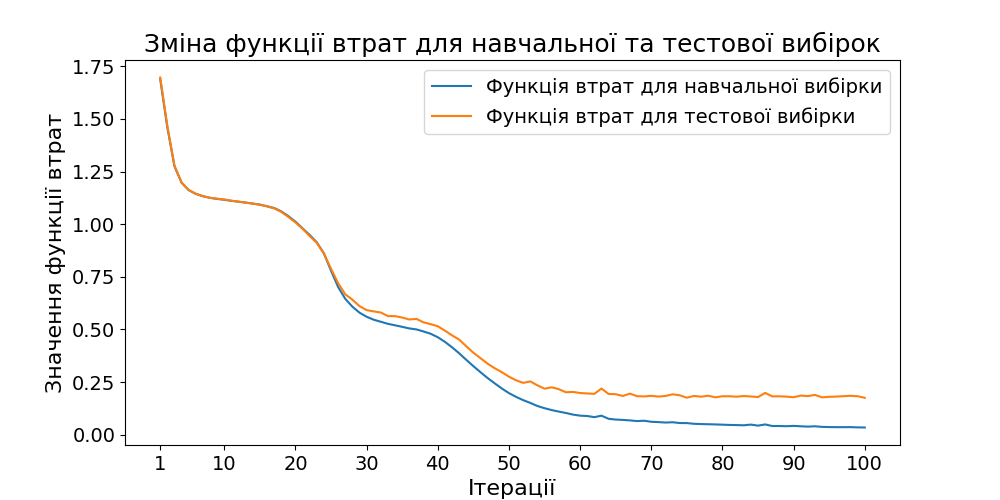
\includegraphics[width=\textwidth]{/home/loipoi/bachelor-diploma/pictures/binary_classification_tabular/mlp_with_gd.png}
		\caption{}
	\end{subfigure}%

	\begin{subfigure}[b]{0.85\textwidth}
		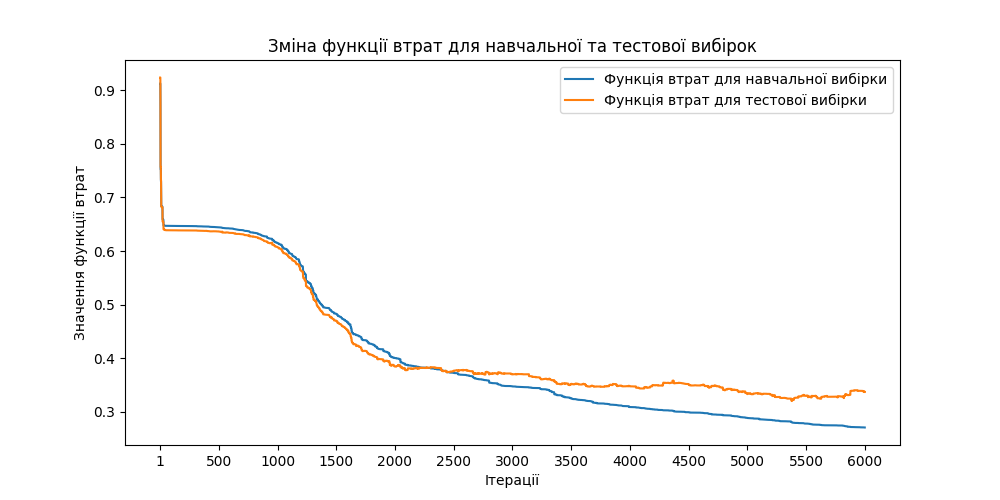
\includegraphics[width=\textwidth]{/home/loipoi/bachelor-diploma/pictures/binary_classification_tabular/mlp_with_spm.png}
		\caption{}
	\end{subfigure}%
	
	\begin{subfigure}[b]{0.85\textwidth}
		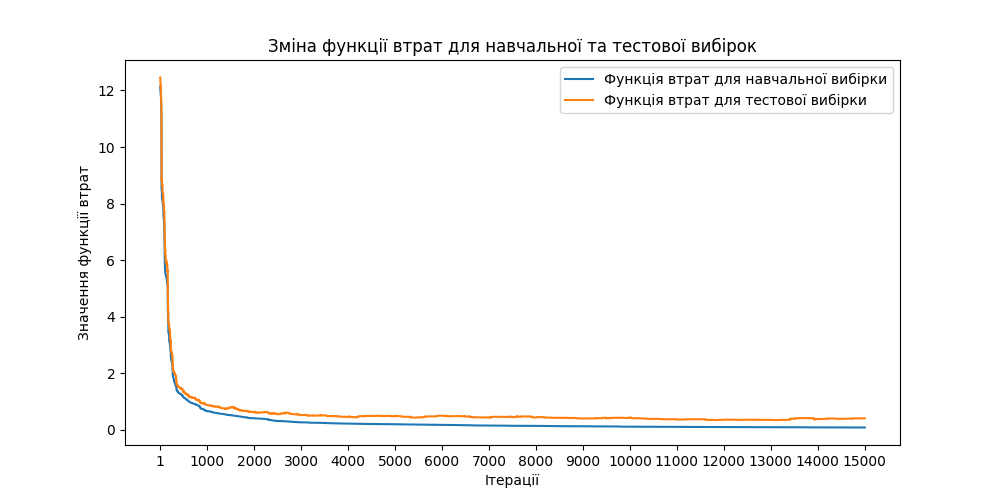
\includegraphics[width=\textwidth]{/home/loipoi/bachelor-diploma/pictures/binary_classification_tabular/ea.png}
		\caption{}
	\end{subfigure}
	
	\caption{Графіки залежності функцій втрат від кількості ітерацій для методу: (a) MLP with gradient descent, (б) MLP with single-point mutation, (в) $(1+\lambda)$-EA with GP encodings}
	\label{fig_losses}
\end{figure}

Як видно з цих даних, усі три моделі можуть досягти приблизно однакових метрик, але якщо говорити в термінах часу, то на цих даних найкраще себе показали моделі MLP with gradient descent та $(1+\lambda)$-EA with GP encodings, час роботи, яких склав 0.6110560894012451 та 0.641812801361084 секунд відповідно, в той час, як алгоритму MLP with single-point mutation знадобилось значно більше часу, щоб зійтися до таких же метрик -- 8.22137975692749 секунд.

Тепер перейдемо до задачі бінарної класифікації картинок. Як ми вже згадували у розділі \ref{sec:data-description} для цього ми використовували датасет Chest X-Ray Images (Pneumonia)~\cite{ct32}. Оптимальні гіперпараметри для усіх трьох моделей можна знайти у попередньому розділі. Зазначимо, що моделі тренувалися протягом 150, 6000 та 70 епох відповідно. Після тренування ми отримали результати для моделі MLP with gradient descent, які можна подивитися в таблиці \ref{mlp_gd_bc_td_results}, для моделі MLP with single-point mutation - у таблиці \ref{mlp_spm_bc_td_results}, для моделі $(1+\lambda)$-EA with GP encodings - у таблиці \ref{ea_bc_td_results}. Результуючі метрики на найкращій ітерації для усіх трьох моделей знаходяться в таблиці \ref{metrics_bc_td_results}. Графіки зміни функцій втрат для кожної моделі можна знайти на рисунку \ref{fig_losses}

\chapconclude{\ref{chap:practice}}

Висновки до останнього розділу є, фактично, підсумковими під усім 
дослідженням; однак вони повинні стостуватись саме того, що розглядалось у 
розділі.